\documentclass{ximera}

\title{Fractions Videos}
\author{Amy Riordan}

\begin{document}
\begin{abstract}
Fractions video resources from Module 1.
\end{abstract}
\maketitle

\section*{Fraction Videos}

Below each video, you’ll find a set of practice problems. Try those problems first. If you run into any difficulties, go back and rewatch the video, then attempt the problems again. This way, you’ll reinforce what you’ve learned and build a stronger understanding.

Fractions (ERAU | 7:00)

\youtube{placeholder}

% filepath: /code/fractions.tex
% ...existing code...

\section*{Identifying Numerator and Denominator}

For each fraction below, identify the numerator and the denominator.

\begin{problem}
\begin{enumerate}
\item The numerator of $\frac{4}{7}$ is \wordChoice{
\choice[correct]{4}
\choice{7}
}
 
\item The denominator is $\frac{3}{5}$ is \wordChoice{
\choice{3}
\choice[correct]{5}
}
 
\end{enumerate}
\end{problem}

% filepath: /code/fractions.tex
% ...existing code...

\section*{Proper and Improper Fractions}

For each fraction below, identify whether it is a proper fraction or an improper fraction.

\begin{problem}
\begin{enumerate}
    \item $\frac{5}{8}$ is a \wordChoice{
        \choice[correct]{proper fraction}
        \choice{improper fraction}
    }
    \item $\frac{9}{4}$ is a \wordChoice{
        \choice{proper fraction}
        \choice[correct]{improper fraction}
    }
    \item $\frac{7}{7}$ is a \wordChoice{
        \choice{proper fraction}
        \choice[correct]{improper fraction}
    }
\end{enumerate}
\end{problem}

% ...existing code...

Mixed Numbers (ERAU| 3:48)

\youtube{placeholder}

% filepath: /code/fractions.tex
% ...existing code...

\section*{Improper Fractions and Mixed Numbers}

\begin{problem}
 
Write a fraction of the shaded portion of the figure as a mixed number and an improper fraction below.
 
\begin{center}
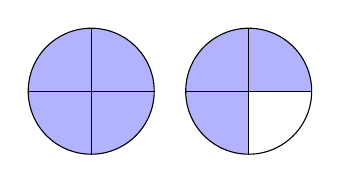
\begin{tikzpicture}[scale=1]
% First circle: all quarters filled
\foreach \i in {0,90,180,270} {
  \begin{scope}
    \clip (0,0) circle (0.8);
    \fill[blue!30] (0,0) -- (\i:0.8) arc (\i:\i+90:0.8) -- cycle;
  \end{scope}
}
\draw (0,0) circle (0.8);
\foreach \i in {0,90,180,270} {
  \draw (0,0) -- (\i:0.8);
}
 
% Second circle: three quarters filled
\foreach \i in {0,90,180} {
  \begin{scope}
    \clip (2,0) circle (0.8);
    \fill[blue!30] (2,0) -- ({2+0.8*cos(\i)},{0.8*sin(\i)}) arc (\i:\i+90:0.8) -- cycle;
  \end{scope}
}
\draw (2,0) circle (0.8);
\foreach \i in {0,90,180,270} {
  \draw (2,0) -- ({2+0.8*cos(\i)}, {0.8*sin(\i)});
}
 
\end{tikzpicture}
\end{center}
 
A fraction that could represent the portion of the shaded area as a mixed number is $\answer{1\frac{3}{4}}$.
 
The fraction representing the shaded portion as an improper fraction is $\frac{\answer{7}}{\answer{4}}$.
 
\end{problem}
 
\begin{problem}
 
Write a fraction of the shaded portion of the figure below.
 
\begin{center}
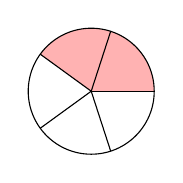
\begin{tikzpicture}[scale=1]
% First circle: 2 fifths filled
\foreach \i in {0,72} {
  \begin{scope}
    \clip (0,0) circle (0.8);
    \fill[red!30] (0,0) -- (\i:0.8) arc (\i:\i+72:0.8) -- cycle;
  \end{scope}
}
\draw (0,0) circle (0.8);
\foreach \i in {0,72,144,216,288} {
  \draw (0,0) -- (\i:0.8);
}
 
\end{tikzpicture}
\end{center}
 
The fraction representing the shaded portion as an proper fraction is $\frac{\answer{2}}{\answer{5}}$.
 
\end{problem}
 
\begin{problem}
 
Write a fraction of the shaded portion of the figure as a mixed number and an improper fraction below.
 
\begin{center}
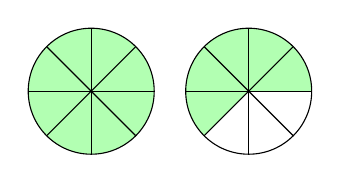
\begin{tikzpicture}[scale=1]
% First circle: all eighths filled
\foreach \i in {0,45,90,135,180,225,270,315} {
  \begin{scope}
    \clip (0,0) circle (0.8);
    \fill[green!30] (0,0) -- (\i:0.8) arc (\i:\i+45:0.8) -- cycle;
  \end{scope}
}
\draw (0,0) circle (0.8);
\foreach \i in {0,45,90,135,180,225,270,315} {
  \draw (0,0) -- (\i:0.8);
}
 
% Second circle: 5 eighths filled
\foreach \i in {0,45,90,135,180} {
  \begin{scope}
    \clip (2,0) circle (0.8);
    \fill[green!30] (2,0) -- ({2+0.8*cos(\i)},{0.8*sin(\i)}) arc (\i:\i+45:0.8) -- cycle;
  \end{scope}
}
\draw (2,0) circle (0.8);
\foreach \i in {0,45,90,135,180,225,270,315} {
  \draw (2,0) -- ({2+0.8*cos(\i)}, {0.8*sin(\i)});
}
 
\end{tikzpicture}
\end{center}
 
A fraction that could represent the portion of the shaded area as a mixed number is $\answer{1\frac{5}{8}}$.
 
The fraction representing the shaded portion as an improper fraction is $\frac{\answer{13}}{\answer{8}}$.
 
\end{problem}
 
\begin{problem}
 
Write a fraction of the shaded portion of the figure below.
 
\begin{center}
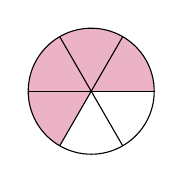
\begin{tikzpicture}[scale=1]
% Single circle: 4 sixths filled
\foreach \i in {0,60,120,180} {
  \begin{scope}
    \clip (0,0) circle (0.8);
    \fill[purple!30] (0,0) -- (\i:0.8) arc (\i:\i+60:0.8) -- cycle;
  \end{scope}
}
\draw (0,0) circle (0.8);
\foreach \i in {0,60,120,180,240,300} {
  \draw (0,0) -- (\i:0.8);
}
 
\end{tikzpicture}
\end{center}
 
The fraction representing the shaded portion as an proper fraction is $\frac{\answer{4}}{\answer{6}}$.
 
\end{problem}
 
\begin{problem}
 
Write a fraction of the shaded portion of the figure as a mixed number and an improper fraction below.
 
\begin{center}
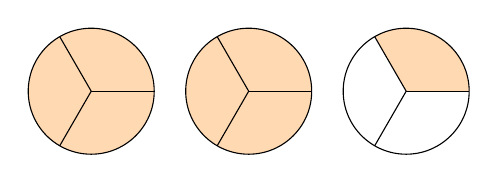
\begin{tikzpicture}[scale=1]
% First circle: all thirds filled
\foreach \i in {0,120,240} {
  \begin{scope}
    \clip (0,0) circle (0.8);
    \fill[orange!30] (0,0) -- (\i:0.8) arc (\i:\i+120:0.8) -- cycle;
  \end{scope}
}
\draw (0,0) circle (0.8);
\foreach \i in {0,120,240} {
  \draw (0,0) -- (\i:0.8);
}
 
% Second circle: all thirds filled
\foreach \i in {0,120,240} {
  \begin{scope}
    \clip (2,0) circle (0.8);
    \fill[orange!30] (2,0) -- ({2+0.8*cos(\i)},{0.8*sin(\i)}) arc (\i:\i+120:0.8) -- cycle;
  \end{scope}
}
\draw (2,0) circle (0.8);
\foreach \i in {0,120,240} {
  \draw (2,0) -- ({2+0.8*cos(\i)}, {0.8*sin(\i)});
}
 
% Third circle: 1 third filled
\begin{scope}
  \clip (4,0) circle (0.8);
  \fill[orange!30] (4,0) -- ({4+0.8*cos(0)},{0.8*sin(0)}) arc (0:120:0.8) -- cycle;
\end{scope}
\draw (4,0) circle (0.8);
\foreach \i in {0,120,240} {
  \draw (4,0) -- ({4+0.8*cos(\i)}, {0.8*sin(\i)});
}
 
\end{tikzpicture}
\end{center}
 
A fraction that could represent the portion of the shaded area as a mixed number is $\answer{2\frac{1}{3}}$.
 
The fraction representing the shaded portion as an improper fraction is $\frac{\answer{7}}{\answer{3}}$.
 
\end{problem}


\section*{Writing Mixed Numbers as Improper Fractions}

For each mixed number below, write it as an improper fraction.

\begin{problem}
$3\frac{2}{5} = \answer{\frac{17}{5}}$
\end{problem}

\begin{problem}
$1\frac{3}{4} = \answer{\frac{7}{4}}$
\end{problem}

\begin{problem}
$5\frac{1}{6} = \answer{\frac{31}{6}}$
\end{problem}

% ...existing code...

% filepath: /code/fractions.tex
% ...existing code...

\section*{Writing Improper Fractions as Mixed Numbers}

For each improper fraction below, write it as a mixed number.

\begin{problem}
$\frac{11}{4} = \answer{2\frac{3}{4}}$
\end{problem}

\begin{problem}
$\frac{17}{5} = \answer{3\frac{2}{5}}$
\end{problem}

\begin{problem}
$\frac{22}{7} = \answer{3\frac{1}{7}}$
\end{problem}

% ...existing code...

Simplifying Fractions (ERAU| 5:17)

\youtube{placeholder}

% filepath: /code/decimals.tex
% ...existing code...

\section*{Prime Factorization}

Find the prime factorization of each number below.

\begin{problem}
$36$.\\
$\answer{2 \cdot 2 \cdot 3 \cdot 3}$
\end{problem}

\begin{problem}
$60$.\\
$\answer{2 \cdot 2 \cdot 3 \cdot 5}$
\end{problem}

\begin{problem}
$84$.\\
$\answer{2 \cdot 2 \cdot 3 \cdot 7}$
\end{problem}

% ...existing code...

% filepath: /code/fractions.tex
% ...existing code...

\section*{Reducing Fractions to Lowest Terms}

For each fraction below, reduce it to its lowest term.

\begin{problem}
$\frac{18}{24} = \answer{\frac{3}{4}}$
\end{problem}

\begin{problem}
$\frac{35}{49} = \answer{\frac{5}{7}}$
\end{problem}

\begin{problem}
$\frac{42}{56} = \answer{\frac{3}{4}}$
\end{problem}

\begin{problem}
$\frac{45}{60} = \answer{\frac{3}{4}}$
\end{problem}

\begin{problem}
$\frac{32}{48} = \answer{\frac{2}{3}}$
\end{problem}

% ...existing code...

Multiplying Fractions (ERAU| 2:57)

\youtube{placeholder}

% filepath: /code/fractions.tex
% ...existing code...

\section*{Multiplying Fractions}

For each problem below, multiply the fractions and write your answer in lowest terms.

\begin{problem}
$\frac{2}{3} \times \frac{4}{5} = \answer{\frac{8}{15}}$
\end{problem}

\begin{problem}
$\frac{3}{7} \times \frac{2}{9} = \answer{\frac{2}{21}}$
\end{problem}

\begin{problem}
$\frac{5}{8} \times \frac{3}{4} = \answer{\frac{15}{32}}$
\end{problem}

\begin{problem}
$\frac{7}{10} \times \frac{5}{14} = \answer{\frac{1}{4}}$
\end{problem}

\begin{problem}
$\frac{9}{11} \times \frac{2}{3} = \answer{\frac{6}{11}}$
\end{problem}

% ...existing code...

Dividing Fractions (ERAU| 4:26)

\youtube{placeholder}

% filepath: /code/fractions.tex
% ...existing code...

\section*{Dividing Fractions}

For each problem below, divide the fractions and write your answer in lowest terms.

\begin{problem}
$\frac{3}{4} \div \frac{2}{5} = \answer{\frac{15}{8}}$
\end{problem}

\begin{problem}
$\frac{7}{9} \div \frac{1}{3} = \answer{\frac{7}{3}}$
\end{problem}

\begin{problem}
$\frac{5}{6} \div \frac{2}{3} = \answer{\frac{15}{12}}$
\end{problem}

\begin{problem}
$\frac{8}{15} \div \frac{4}{5} = \answer{\frac{2}{3}}$
\end{problem}

\begin{problem}
$\frac{9}{10} \div \frac{3}{5} = \answer{\frac{3}{2}}$
\end{problem}

% ...existing code...

Adding and Subtracting Fractions (ERAU| 6:22)

\youtube{placeholder}

% filepath: /code/fractions.tex
% ...existing code...

\section*{Adding and Subtracting Fractions}

For each problem below, add or subtract the fractions and write your answer in lowest terms.

\begin{problem}
$\frac{1}{4} + \frac{1}{2} = \answer{\frac{3}{4}}$
\end{problem}

\begin{problem}
$\frac{1}{3} - \frac{5}{6} = \answer{-\frac{1}{2}}$
\end{problem}

\begin{problem}
$\frac{2}{5} + \frac{3}{10} = \answer{\frac{7}{10}}$
\end{problem}

\begin{problem}
$\frac{7}{8} - \frac{1}{4} = \answer{\frac{5}{8}}$
\end{problem}

\begin{problem}
$\frac{3}{7} + \frac{2}{7} = \answer{\frac{5}{7}}$
\end{problem}

% ...existing code...

Fractions and Decimals (ERAU|7:02)

\youtube{placeholder}

% filepath: /code/fractions.tex
% ...existing code...

\section*{Writing Fractions as Decimals}

For each fraction below, write it as a decimal.

\begin{problem}
$\frac{1}{2} = \answer{0.5}$
\end{problem}

\begin{problem}
$\frac{3}{4} = \answer{0.75}$
\end{problem}

\begin{problem}
$\frac{2}{5} = \answer{0.4}$
\end{problem}

\begin{problem}
$\frac{7}{10} = \answer{0.7}$
\end{problem}

\begin{problem}
$\frac{5}{8} = \answer{0.625}$
\end{problem}

% ...existing code...

Percents, Decimals, and Fractions (ERAU|8:14)

\youtube{placeholder}

Percents, Decimals, and Fractions (Part 2) (ERAU|9:35)

\youtube{placeholder}

% filepath: /code/fractions.tex
% ...existing code...

\section*{Writing Percents as Decimals}

For each percent below, write it as a decimal.

\begin{problem}
$25\% = \answer{0.25}$
\end{problem}

\begin{problem}
$60\% = \answer{0.6}$
\end{problem}

\begin{problem}
$7.5\% = \answer{0.075}$
\end{problem}

% ...existing code...

% filepath: /code/fractions.tex
% ...existing code...

\section*{Writing Decimals as Percents}

For each decimal below, write it as a percent.

\begin{problem}
$0.4 = \answer{40\%}$
\end{problem}

\begin{problem}
$0.75 = \answer{75\%}$
\end{problem}

\begin{problem}
$0.08 = \answer{8\%}$
\end{problem}

% ...existing code...

% filepath: /code/fractions.tex
% ...existing code...

\section*{Writing Fractions as Percents}

For each fraction below, write it as a percent.

\begin{problem}
$\frac{1}{4} = \answer{25\%}$
\end{problem}

\begin{problem}
$\frac{3}{5} = \answer{60\%}$
\end{problem}

\begin{problem}
$\frac{7}{10} = \answer{70\%}$
\end{problem}

% ...existing code...

\end{document}
